\documentclass[a4paper, 12pt]{article}%тип документа

%отступы
\usepackage[left=2cm,right=2cm,top=2cm,bottom=3cm,bindingoffset=0cm]{geometry}

%Русский язык
\usepackage[T2A]{fontenc} %кодировка
\usepackage[utf8]{inputenc} %кодировка исходного кода

%Вставка картинок
\usepackage{wrapfig}
\usepackage{graphicx}
\graphicspath{{pictures/}}
\DeclareGraphicsExtensions{.pdf,.png,.jpg}

%Графики
\usepackage{multirow}
\usepackage{pgfplots}
\pgfplotsset{compat=1.9}

%Математика
\usepackage{amsmath, amsfonts, amssymb, amsthm, mathtools}

%Заголовок
\author{Sifat Md Abdullah Al Hasib \\
Faculty of Physical and Quantum Electronics \\
GROUP Б04-105}
\title{\textbf{QUESTION OF CHOICE \\ 
Experimental Model for Measuring Thermal Conductivity Using Hot Wire Method}}
\begin{document}
\maketitle
\begin{abstract}
Heat flux $J_r$ has a relation with the given heat to the system. From this relationship, I concluded a formula from which we can find the thermal conductivity. In this paper, I explained a little experiment regarding the theory and later I described an important application of this technique is in the Pirani gauge, which is commonly used in vacuum
systems to measure pressure.
\end{abstract}
\section{General Theory}
We can defined heat as thermal energy in transit. It quantifies the
transfer of energy in response to a temperature gradient. The amount
of heat that flows along a temperature gradient depends on the thermal
conductivity of the material, which we will now define. Thermal conductivity can be considered in one dimension using the
diagram shown in Fig.1. Heat flows from hot to cold, and so flows
against the temperature gradient. The flow of heat can be described by
a heat flux vector J, whose direction lies along the direction of flow of heat and whose magnitude is equal to the heat energy flowing per unit
time per unit area (measured in $Js^{-1}m^{-2} = Wm^{-2}$). The heat flux $J_z$ in the z-direction is given by
\begin{center}
$J_z = -\kappa(\frac{\partial T}{\partial z})$
\end{center}

where the negative sign is because heat flows downhill. The constant
$\kappa$ is called the thermal conductivity of the gas. In general, in three dimensions we can write that the heat flux $J$ is related to temperature using
\begin{center}
$J = -\kappa \nabla T$
\end{center}

\begin{figure}[h]
\begin{center}
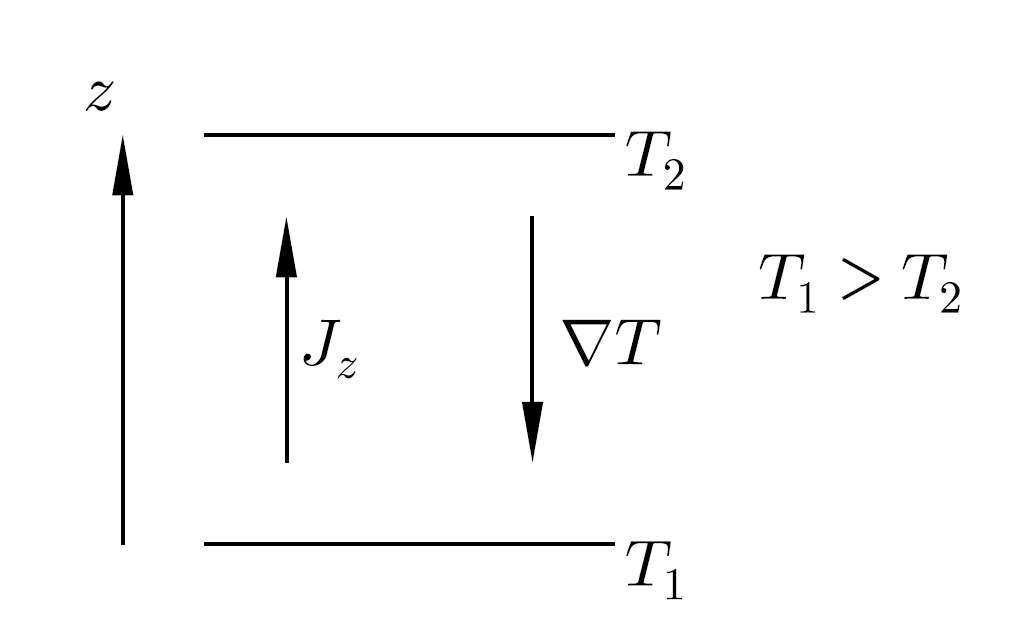
\includegraphics[width = 0.8\textwidth]{Bigar 1.png}
\caption{Heat flows in the opposite direction to the temperature gradient.}
\end{center}
\end{figure}
\newpage
\section{Measurement of Thermal Conductivity} 
The thermal conductivity $\kappa$ can be measured using the hot wire method. Gas fills the space between two coaxial cylinders (inner cylinder radius a, outer cylinder radius b) as shown in Fig.2. The outer cylinder is connected to a constant-temperature bath of temperature $T_b$, while heat is generated in the inner cylinder (the hot wire)at rate Q per unit length of the cylinder (measured in units of $ Wm^{-1}$. The temperature of the inner cylinder rises to $T_a$. The rate $Q$ can be connected with the radial heat flux $J_r$ using

\begin{center}
$Q = 2 \pi r J_r$
\end{center}
and $J_r$ itself is given by $-\kappa \frac{\partial T}{\partial r}$ as in the first equation. Hence,
\begin{center}
$Q = {-2} \pi r \kappa \frac{\partial T}{\partial r} $
\end{center}
Rearranging and integrating yields
\begin{center}

$Q \int_{a}^{b} \frac{dr}{r} = -2\pi\kappa\int_{T_a}^{T_b}dT $
\end{center}
and hence
\begin{center}
$\kappa = \frac{Q}{2\pi}\frac{ln(b/a)}{T_a - T_b} $
\end{center}
Since $Q$ is known (it is the power supplied to heat the inner cylinder) and $T_a$ and $T_b$ can be measured, the value of $\kappa$ can be deduced.
\begin{figure}[h]
\begin{center}
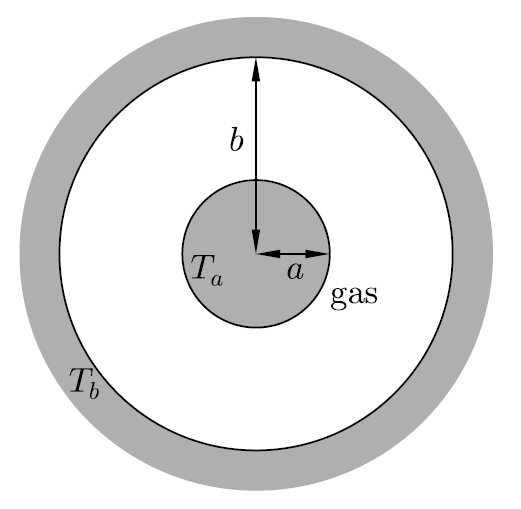
\includegraphics[width = 0.8\textwidth]{B3.png}
\caption{The hot-wire method for measuring thermal conductivity}
\end{center}
\end{figure}
\newpage
\section{Pirani Gauge} The Pirani gauge is a robust thermal conductivity gauge used for the measurement of the pressures in vacuum systems. It was invented in 1906 by Marcello Pirani An important application of this technique is in the Pirani gauge, which is commonly used in vacuum systems to measure pressure. A sensor wire is heated electrically, and the pressure of the gas is determined by measuring the current needed to keep the wire at a constant temperature. (The resistance of the wire is temperature dependent, so the temperature is estimated by measuring the resistance of the wire.) The Pirani gauge thus relies on the fact that at low pressure the thermal conductivity is a function of pressure (since the condition $\lambda \ll L$, where $L$ is a linear dimension in the gauge, is not met). In fact, a typical Pirani gauge will not work to detect pressures much above 1 mbar because, above these pressures, the thermal conductivity of the gases no longer changes with pressure. The thermal conductivity of each gas is different, so the gauge has to be calibrated for the individual gas being measured. In the picture below I just give a photo of the block diagram of Pirani gauge without detailed discussion. 
\begin{figure}[h]
\begin{center}
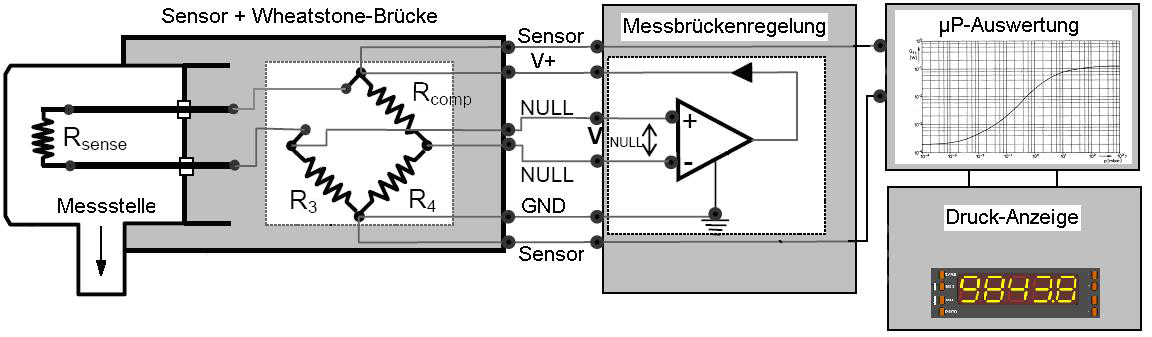
\includegraphics[width = 0.8\textwidth]{B2.png}
\caption{Block diagram of Pirani gauge}
\end{center}
\end{figure}
\newpage
\section{Conclusion} 
We can find the thermal conductivity using different method. Among them hot wire method has very practical uses. I just showed the main scheme of the experiment in figure 2. When we will do experiment, we should measure the radius of two cylinder and the temperature of outer cylinder first and decided that how many heat we will give to the system. Then we can get a tabular value of heat conductivity then we can compare what we get from our experiment. Here we should consider the metal of which the cylinder are made. 


\end{document}